%------- Generic settings
\documentclass[10pt,oneside,a4paper]{article} 

\usepackage[a4paper, 
            left=2.0cm, 
            right=1.7cm, 
            top=3cm, 
            bottom=2.0cm,
            marginparwidth=1cm]{geometry}
% following two lines suggested by Joh Kitchin 
% for writing nice documents with well-spaced lines
\usepackage{setspace}
\onehalfspacing

\setlength{\parindent}{20pt}
\usepackage[utf8]{inputenc}
\usepackage{amsthm,amsmath,amssymb,amsfonts}
\usepackage{csquotes}
\usepackage{titling}
\setlength{\droptitle}{-60pt}
\usepackage{marginnote}
% to take away the error unknown float option `H'
\usepackage{float}             
% Making caption font smaller on figures and tables.  
% https://stackoverflow.com/a/27243065/505306
\usepackage{caption} 
\captionsetup{font=footnotesize}
\usepackage[framemethod=TikZ]{mdframed}
\usepackage{tocloft}
% Adding a line at the top of the table of contents saying page
\addtocontents{toc}{~\hfill\textbf{Page}\par}
\renewcommand\cftsecleader{\cftdotfill{\cftdotsep}}
\usepackage[titletoc,toc,page]{appendix}
% The great microtype package for better word adjustment 
%https://tex.stackexchange.com/a/586  
\usepackage[stretch=10]{microtype} 
% For aligning itemize environments to left 
% https://tex.stackexchange.com/a/278199/17858
\usepackage{enumitem}               
% if you want to create a new list from scratch  
% https://tex.stackexchange.com/q/2291/17858
\newlist{alphalist}{enumerate}{1}      
% in that case, at least label must be specified using \setlist
\setlist[alphalist,1]{label=\textbf{\Alph*.}} 
\usepackage[english]{babel}
\setlength{\headsep}{5pt}
\usepackage{blindtext,kantlipsum}
\usepackage{mathtools}
\usepackage{listings}
\usepackage[inline]{asymptote}
\usepackage{asypictureB}
\usepackage{filecontents}
\usepackage{parskip} 
\usepackage{tikz,graphicx}                            
% For lists in two or more columns
\usepackage{multicol}  
\usepackage[nokwfunc, ruled]{algorithm2e}
\newcommand\mycommfont[1]{\footnotesize\ttfamily\textcolor{blue}{#1}}
\usepackage[T1]{fontenc}
% So that sections/code-blocks don't straddle two pages 
\usepackage{needspace}  
\usepackage{mathtools}
\usepackage{subfig}
\usepackage{etoolbox}
\usepackage{color}
\usepackage{pifont}
% For italicizing quotes: https://tex.stackexchange.com/a/288556/17858, 
% from https://tex.stackexchange.com/a/391739
\usepackage{quoting,xparse} 
\NewDocumentCommand{\bywhom}{m}{% the Bourbaki trick
  {\nobreak\hfill\penalty50\hskip1em\null\nobreak
   \hfill\mbox{\normalfont(#1)}%
   \parfillskip=0pt \finalhyphendemerits=0 \par}%
}
\NewDocumentEnvironment{pquotation}{m}
  {\begin{quoting}[
     indentfirst=true,
     leftmargin=\parindent,
     rightmargin=\parindent]\itshape}
  {\bywhom{#1}\end{quoting}}
% Convenience commands
\newcommand*\circled[1]{\tikz[baseline=(char.base)]{\node[shape=circle,draw,inner sep=2pt] (char) {#1};}}
\providecommand{\myceil}[1]{\left \lceil #1 \right \rceil }	    % Ceil function
% Floor function\renewcommand{\labelitemi}{\tiny$\blacksquare$}	
\providecommand{\myfloor}[1]{\left \lfloor #1 \right \rfloor }
% for drawing the conditional probability `|` sign neatly.
\newcommand\given[1][]{\:#1\vert\:} 
\newcommand\RR{\mathbb{R}}				
\newcommand\CC{\mathbb{C}}			
\newcommand\ZZ{\mathbb{Z}}		
\newcommand\NN{\mathbb{N}}	
\newcommand\rarr{\rightarrow}
\newcommand\larr{\leftarrow}	
\newcommand\defeq{\coloneqq}% := symbol
\renewcommand\tilde{ \: \thicksim \: }% Sane tildas
\newmdenv[topline=false, 
	  bottomline=false, 
	  skipabove=\topsep,
	  skipbelow=\topsep]{siderules}
% https://tex.stackexchange.com/a/458876/17858 
% rounded pink rectangles around an inline word
\newcommand{\sticker}[1]{\tikz[baseline=(X.base)]
	                 \node [draw=red,
			 	fill=pink!60,
				semithick,
                                rectangle,
				inner sep=2pt, 
				rounded corners=3pt](X){{\footnotesize \color{red} #1}};} 
\newif\ifshowcode
\showcodetrue
\usepackage{latexsym}
\usepackage{listings}
\usepackage{color}
\definecolor{linkcolor}{rgb}{0.1, 0.60, 0.20}
\usepackage{todonotes}
\usepackage{booktabs}
\usepackage[%
      raiselinks,%
      pdfhighlight=/O,%
      hyperfigures,%
      breaklinks,%
      colorlinks,%
      pdfstartview=FitBH,%
      linkcolor={linkcolor},%
      anchorcolor={linkcolor},%
      citecolor={linkcolor},%
      filecolor={linkcolor},%
      menucolor={linkcolor},%
      urlcolor={linkcolor}%
   ]{hyperref}
% Taken from https://tex.stackexchange.com/a/371469 
% for drawing a nice rule across the page
\newcommand\myrule{\par\noindent\rule{\textwidth}{0.4pt}}
\usepackage{xcolor}
\usepackage{sectsty}
%\allsectionsfont{\sffamily}
\definecolor{lava}{rgb}{0.81, 0.06, 0.13}
\definecolor{mahogany}{rgb}{0.75, 0.25, 0.0}
\definecolor{sacramentostategreen}{rgb}{0.0, 0.34, 0.25}
\setcounter{tocdepth}{2}
\usepackage{marginnote}
\newcommand\margin[1]{\marginnote{\color{cadmiumgreen}{#1} }}
\definecolor{cadmiumgreen}{rgb}{0.0, 0.42, 0.24}
% Squaremarkers for bullets of itemized lists
\usepackage{wasysym}
\usepackage{marvosym}
%\renewcommand{\labelitemi}{\scriptsize$\blacksquare$}
\renewcommand{\labelitemi}{\ding{118}} % 4 squares in the form of a diamond
% To express an idea in a crunchy way.
\newcommand{\crunchy}[1]{\lbrack{} \large \textit{#1} \normalsize \rbrack}
% For commenting out block of text, that you still 
% want syntax highlighted in the LaTeX file
\newcommand{\remove}[1]{} 
% For page numbers at top right. Found this here
% https://tex.stackexchange.com/a/56321
\pagestyle{myheadings}
% For left aligning title and authors
% https://tex.stackexchange.com/q/85343
\makeatletter
\usepackage[us,12hr]{datetime}
\renewcommand{\maketitle}{\bgroup\setlength{\parindent}{0pt}
\begin{flushleft}
  \textbf{\LARGE \@title} \\ \vspace{2mm} 
  \large \@author  \\ \vspace{3.5mm} 
  \large \@date{} \\
  \currenttime \normalsize
\end{flushleft}\egroup
}
\makeatother
% https://tex.stackexchange.com/a/192504 
% Force itemize inside description onto a new line
\setlist[itemize]{topsep=0pt,before=\leavevmode\vspace{-1.5em}}
\setlist[description]{style=nextline}
% For highlighting options to programs 
% according to man-pages.
\definecolor{optcol}{rgb}{0.70, 0, 0}
\newcommand{\opt}[1]{{\color{optcol}\textit{\texttt{#1}}}}

\usepackage{noweb}
%------- Bibtex
\usepackage[backend=bibtex, style=alphabetic, sorting=none]{biblatex}
%\setlength\bibitemsep{\baselineskip}
\addbibresource{References.bib}
%------- Title
\usepackage{longfbox}
\title{\Huge \lfbox[background-color=green!10,border-width=0.00pt]{Conical Routing For Lookahead}}
\author{\Large Gaurish Telang \\ 
       \Large \href{mailto:gaurish108@gmail.com}{\texttt{gaurish108@gmail.com}}}
%------- Top right picture, a picture representative of the program to be implemented, 
\usepackage{eso-pic}
%\AddToShipoutPicture*
%    {\put(365,610){\frame{\includegraphics[width=5.40cm]{miscimages/pitbull.png}}}}
%-------- Coloring section titles
\usepackage{xcolor,titlesec}
\titleformat{name=\section}[block]
  {\scshape\rmfamily\Large}
  {}
  {0pt}
  {\colorsection}
\titlespacing*{\section}{0pt}{\baselineskip}{\baselineskip}
\newcommand{\colorsection}[1]{%
  \colorbox{green!10}{\parbox{\dimexpr\textwidth-2\fboxsep}{\thesection\;\; #1}}}
%-------- Indices
\usepackage[utf8]{inputenc}
\usepackage[T1]{fontenc}
\usepackage{imakeidx}
\makeindex[columns=3, title=\fbox{Index}, intoc]
%-------------------------------------------------------------------------------
\begin{document}
\maketitle
% Man-page and TOC
%\vspace{5mm}
\begin{description}
  \item[NAME] {\tt ls} - list directory contents
  \item[SYNOPSIS]  List  information  about the FILEs (the current directory by default).  
                   Mandatory arguments to long options are mandatory for short options too.
  \item[DESCRIPTION] \kant[1]
  \item[OPTIONS]
     \begin{description}
        \item[\opt{-a, --all}]
              do not ignore entries starting with .
        \item[\opt {-A, --almost-all}]
              do not list implied . and ..
       \item[\opt{ --author}]
              with {\tt -l}, print the author of each file
       \item[\opt{ -h, --human-readable}]
              with \opt{-l} and/or \opt{-s}, print human readable sizes 
     \end{description}
  \item[EXIT STATUS]
     \begin{itemize}
       \item[\tt{0}] if OK
       \item[\tt{1}] if minor problems (e.g. cannot access subdirectory)
       \item[\tt{2}] if serious trouble (e.g. cannot access command-line argument)
     \end{itemize}    
  \item [QUICK INSTALLATION INSTRUCTIONS] Mention what is required for the code to run, what libraries                                                                                                  
        and links to download sites. The list of dependencies can be extracted                                                                                        
        by using AWK on the files, alternatively, keep a running tag of                                                                                               
        libraries used, by adding to a separate Index which remembers what                                                                                            
        software was used. For C\texttt{++} programs, all you would have to do                                                                                        
        once the dependencies are installed to type make. Alternatively                                                                                               
        you can also provide a configur script for a larger program.                                                                                                  
        Even better just give them your docker container and tell them                                                                                                
        how to execute the program via the docker container. The docker                                                                                                
        container should be minimal, skeletal actually so that it does                                                                                                
        not take up disk space. Thus this must contain short installation                                                                                              
        instructions.   
\end{description}
 \newpage
\tableofcontents
% Begin main contents
\nwfilename{mainlitprog.nw}\nwbegindocs{0}\section{Introduction}% ===> this file was generated automatically by noweave --- better not edit it




\begin{figure}[H]
\centering
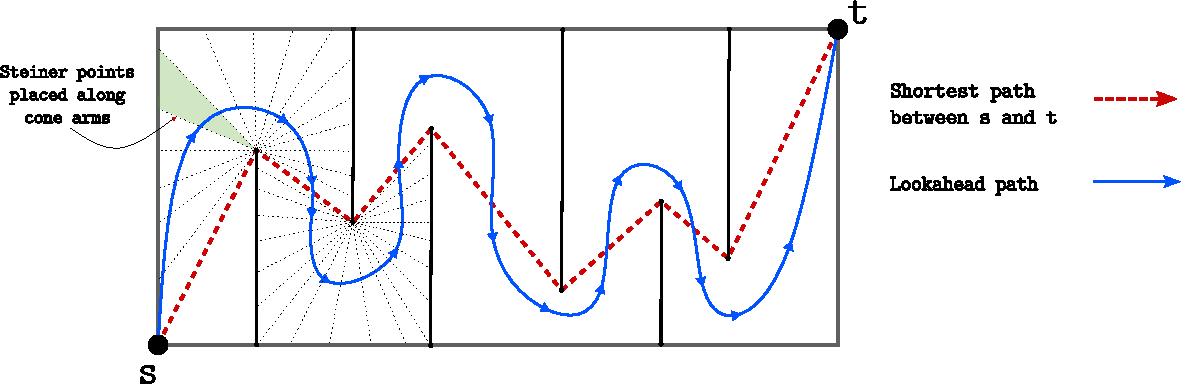
\includegraphics[width=16cm]{miscimages/stalactites-stalagmites.pdf}
\caption{Conical Routing between start $s$ and destination $t$}
\label{fig:conical-routing}
\end{figure}



This document presents a scheme  to solve the lookahead problem 
in the `stalactite and stalagmite' setting using a method based on discretizing the space into a sequence of cones. 
The hope is that, at least experimentally, this scheme will lead to short lookahead paths where each point along the 
curve can see a sufficient chunk of the curve immediately ahead of it. \footnote{We are using Euclidean visibility here
where a point $A$ sees another point $B$ iff the line segment AB is contained in the closure of the free space. }


The basic idea is captured in \autoref{fig:conical-routing}:

Since this document is meant to be a proof-of-concept, for the scheme I will 
use the following simplifying assumptions: stalactites and stalagmites 
alternate in their placement and that their arrangement is such that the shortest path between 
$s$ and $t$ is taut against their tips. 



The scheme is based on the intuition that if the string length upper bounded by a number 
\footnote{say $O(1)L$, where $L$ is the length of the shortest path between $s$ and $t$, 
          such as the red path in \autoref{fig:conical-routing}}
maximizing lookahead is equivalent to  we need to either maximizing minimum 
amount of path string in each cone (or alternatively in each line). 

Then to get the shortest path with the specified amount of lookahead we just do a binary or parametric search 
over different string lengths to find the smallest string length that does not violate the given lookahead bound. 

For the scheme 

\begin{itemize}
 \item Consider a finite sequence of small angles $\Delta \theta_i, 0 \leq i \leq N$, where $N \rightarrow \infty$,  such that 
      $\sum \Delta \theta_i =  $ reflex angle between successive segments (red segments in \autoref{fig:geomdisc}) of a shortest path incident at an 
       obstacle tip . We draw cones of angles $\Delta \theta_i, i \in \mathbb{N}$ generated by a rocking line at each stalactite and stalagmite tip 
       between these shortest path segments. In \autoref{fig:geomdisc} the area not swept by the line during its motion is a wedge facing upward (colored green).  
       Note that the green wedge itself is discretized into small cones as part of the cone sequence just mentioned. 
\item Place Steiner points separated by a small distance $\Delta x$ starting from the obstacle segment tip along each arm of every cone, for as long as the cone arm lies inside free space.
\item Draw the complete bipartite graph between the Steiner points of each cone  as shown in \autoref{fig:geomdisc}
 \item Solve the following linear program, imposing any natural shape constraints  if required.
\end{itemize}

\begin{figure}
    \centering
    \subfloat[A rocking line (blue) creates a sequence of cones of angles 
     $\Delta \theta_i$ between two successive shortest path edges]{{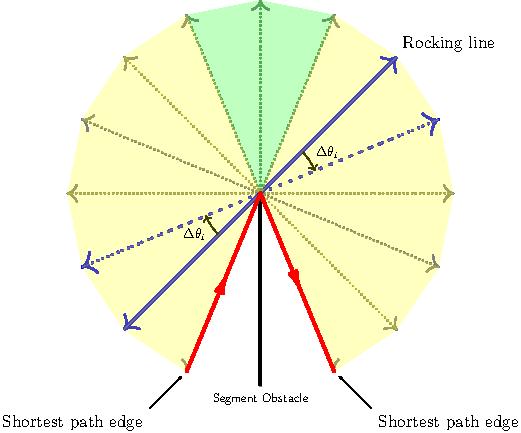
\includegraphics[width=11cm]{asy2d/rocking-line.pdf} }}
    \qquad
    \subfloat[Complete bipartite graph (green) between points on two arms of a cone on the Steiner points. 
              Distance between two consecutive Steiner points along each arm is $\Delta x$. $O$ is the tip of the 
      stalactite/stalagmite.]{{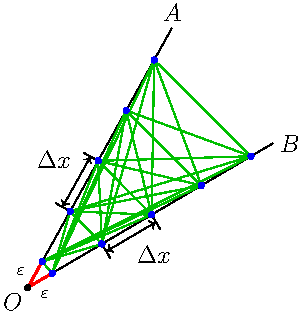
\includegraphics[width=7cm]{asy2d/bipartite-cone.pdf} }}
    \caption{Geometry of the discretization in the neighborhood of each stalactite/stalagmite tip}
    \label{fig:geomdisc}
\end{figure}

Heavy use of the CGAL kernel via its Python bindings have been made in the code which implements the scheme above to ensure
all geometric computations are precise. 

\nwenddocs{}



% Bibliography, appendices and index
\printbibliography
%\begin{appendices}
\renewcommand{\thesection}{\Roman{section}\;\;}
\section{Complete installation instructions}
\subsection{On GNU/Linux systems}
\blindtext
\subsection{Windows 10 + Cygwin}
In this example several keywords\index{keywords} will be used 
which are important and deserve to appear in the Index\index{Index}.
Terms like generate\index{generate} and some\index{others} will also 
show up. Terms in the index can also be nested \index{Index!nested}

\section{Reading Chunk numbers}

From left to right. This is how you should learn to read numbers generated 
by noweb when definiing a new or extending a chunk. 

\section{Layout of source files}
Generate this using some bash commands to give overview of the 
project tree. 


\end{appendices}

%\newpage
%\printindex
\end{document}
